\section{Probabilistic Particle Tracing Model}

In order to analyze the uncertain flow field by particle tracing, in this section we introduce our probability-based particle tracing model. First, we describe the global modeling of streamlines and how to estimate the trace distributions for a given distribution data. Then local distributions used by the global model are detailed.

\subsection{Global Modeling}

Single streamline $L$ originating from position ${x_0}$ can be modeled as $L = \{ {x_0},{x_1},...,{x_n}\} = {x_{0:n}}$, where $x_t$ refers to a position in $\mathrm{R}^d$. As mentioned by Otto et al. in~\cite{Otto10a, Otto11a}, conventional streamline integration methods such as RK4 are not well defined for uncertain vector fields, since there is no unique vector direction at a location ${x_t}$. Therefore, as with most previous methods~\cite{Otto10a, Otto11a}, we make use of the Euler integration model in this paper:
\begin{equation}
  {x_{t + 1}} = {x_t} + {v_t}\Delta t
\end{equation}
where ${v_t}$ and $\Delta t$ refer to the vector direction and the step size at step $t$. Since we focus on generating streamlines from steady vector fields in this work, it is safe to ignore the magnitude of the vectors. And if we set the step size $\Delta t$ as a constant, we can represent the streamline by a sequence of vector directions ${L = v_{0:n}}$, since the streamline trajectory only depends on the propagation directions $v_{0:n}$.

For the uncertain vector fields, there is no unique streamline $v_{0:n}$ for a given starting point $x_0$. Let $\Omega_{x_0}$ be the set of all possible streamlines which originate from $x_0$ given the uncertain data $\mathcal{H}$, we then can define a probability density function (pdf) over the path space, which is:
\begin{equation}
  p(v_{0:n}|\mathcal{H})
\end{equation}
where $\mathcal{H}$ is the set of observations from the uncertain data along the streamline trajectory. Here, we denote the distribution obtained at the starting point $x_t$ of a vector $v_t$ as $\lambda_t=\mathcal{H}(v_t)$. By applying the Bayes theorem, the target distribution $p({v_{0:n}}|{\lambda_{0:n}})$ can be represented by the prior density $p({v_{0:n}})$ and the conditional observation density $p({\lambda_{0:n}}|{v_{0:n}})$, as:
\begin{equation}
  p({v_{0:n}}|{\lambda_{0:n}}) = \frac{{p({v_{0:n}})p({\lambda_{0:n}}|{v_{0:n}})}}{{p({\lambda_{0:n}})}}
\end{equation}
where ${p({\lambda_{0:n}})}$ is a normalizing constant for a fixed data realization, which equals to $\int {p({v_{0:n}},{\lambda_{0:n}})} d{v_{0:n}}$.

Scientific simulations commonly represent physical phenomena as continuous functions. Thus, the sequence of vector directions $v_{0:n}$ along the particle trace should be correlated. This constraint can be modeled as a conditional prior density $p({v_t}|{v_{0:t - 1}})$. In this paper, we assume the sequence $v_{0:n}$ forms a Markov chain, which means the vector direction $v_t$ only depends on the previous direction $v_{t-1}$, but not on $v_{t-2},...,v_0$; so:
\begin{equation}
  p({v_t}|{v_{0:t - 1}}) = p({v_t}|{v_{t - 1}})
\end{equation}
where $p({v_t}|{v_{t - 1}})$ denotes the probability density associated with the transition from $v_{t - 1}$ to $v_t$. Hence, the probability density for a given streamline can be formulated as:
\begin{equation}
  p({v_{0:n}}) = p({v_0})\prod\limits_{t = 1}^n {p({v_t}|{v_{t - 1}})}
\end{equation}
where $p(v_0)$ can be defined by a uniform distribution, since no prior knowledge is applied.

By measuring the observations $\lambda_{0:n}$ along a given streamline $v_{0:n}$, we can get the conditional observation density $p({\lambda_{0:n}}|v_{0:n})$, which defines a measure of how the observations match the given path. In the other word, the observation density gives how likely the distributions $\lambda_{0:n}$ will be observed if the given streamline $v_{0:n}$ actually exists in the flow field. Likewise, we assume that the observation measured at a point does not depend on any previous points in the trace, i.e.:
\begin{equation}
  p(\lambda_t|v_{0:t}) = p({\lambda_t}|{v_t})
\end{equation}
which defines the likelihood density:
\begin{equation}
  p({\lambda_{0:n}}|{v_{0:n}}) = \prod\limits_{t = 0}^n {p({\lambda_t}|{v_t})}
\end{equation}

By substituting (5) and (7) into (3), the posterior density $p({v_{0:n}}|{\lambda_{0:n}})$ can be expanded as:
\begin{equation}
  p({v_{0:n}}|{\lambda_{0:n}}) = \frac{{p({v_0})\prod\limits_{t = 1}^n {p({v_t}|{v_{t - 1}})} \prod\limits_{t = 0}^n {p({\lambda_t}|{v_t})} }}{{p({\lambda_{0:n}})}}
\end{equation}

Since $p({v_{0:n}}|{\lambda_{0:n}})$ is high-dimensional, non-standard, and only known up to a proportionality constant, which makes it infeasible to be evaluated in closed-form. Therefore, a Monte Carlo based method needs to be used to approximate the target distribution. In this case, particle filtering~\cite{doucet2001sequential} as one of Sequential Monte Carlo methods is suitable to approximate the target distribution in iterations. We first put a number of weighted particles at the seed position and update them iteratively. At each iteration, the vector directions which the particles will propagate along with are sampled from an importance function. Then the weight of each particle can be updated based on the importance sampling. Furthermore, the particles can be resampled based on their weights. In the end, a set of weighted particle tracing are obtained to represented the target posterior distribution, from which the most likely trace can be chosen by maximum a posteriori estimation (MAP) estimation.

\subsection{Local Modeling}

In this section, we will elaborate how to model and estimate the local densities in detail.

\noindent\textbf{Prior Density.} As mentioned before, prior density is used to characterize the correlation between two adjacent vector directions. In this work, a prior density which prefers to continue in the previous direction and gives decreasing probability for sharper turns is used. As presented by Zhang et al. in~\cite{Zhang20095}, the von Mises-Fisher distribution~\cite{fisher} has been selected as the prior density due to its mathematical simplicity and tractability.

For a random $d$-dimensional unit vector $v$ on the $(d-1)$-dimensional sphere, with respect to the mean direction $\mu$ and the concentration parameter $\kappa$, the probability density function of the von Mises-Fisher distribution is given by
\begin{equation}
  f_{d}(v| \mu, \kappa)=C_{d}(\kappa)\exp \left( {\kappa \mu^T v } \right)
\end{equation}
where the normalization constant $C_{d}(\kappa)\,$ is
\begin{equation}
  C_{d}(\kappa)=\frac {\kappa^{d/2-1}} {(2\pi)^{d/2}I_{d/2-1}(\kappa)} \,
\end{equation}
in which $I_{d/2-1}$ denotes the modified Bessel function of the first kind and order $d/2-1$.

The parameter $\kappa$ defined in range $\kappa \ge 0$ is used to control the concentration of the distribution around the mean direction $\mu$. The distribution with higher concentration will have a greater $\kappa$ value. Figure~\ref{fisher} gives examples of points sampled from 2-dimensional von Mises-Fisher distributions with different $\kappa$.

\begin{figure}[htb]
  \centering
  \begin{subfigure}[b]{0.16\textwidth}
    \centering
    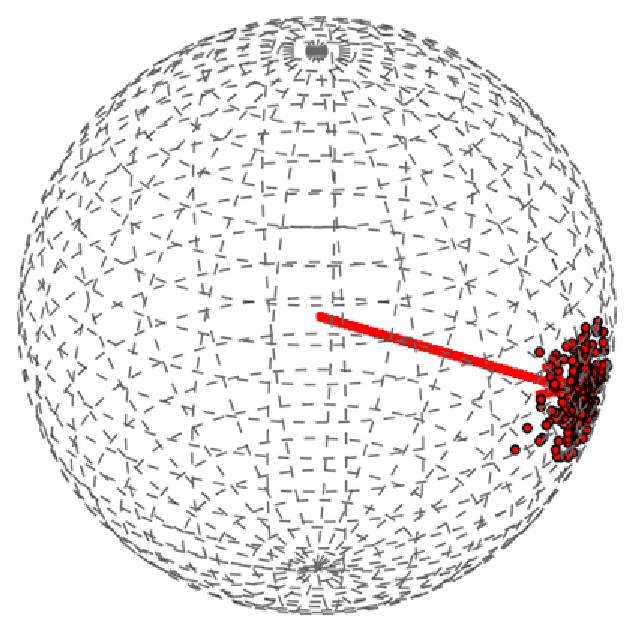
\includegraphics[width=0.8in]{../figures/vf_100.eps}
    \caption{$\kappa=100$}
  \end{subfigure}~
  \begin{subfigure}[b]{0.16\textwidth}
    \centering
    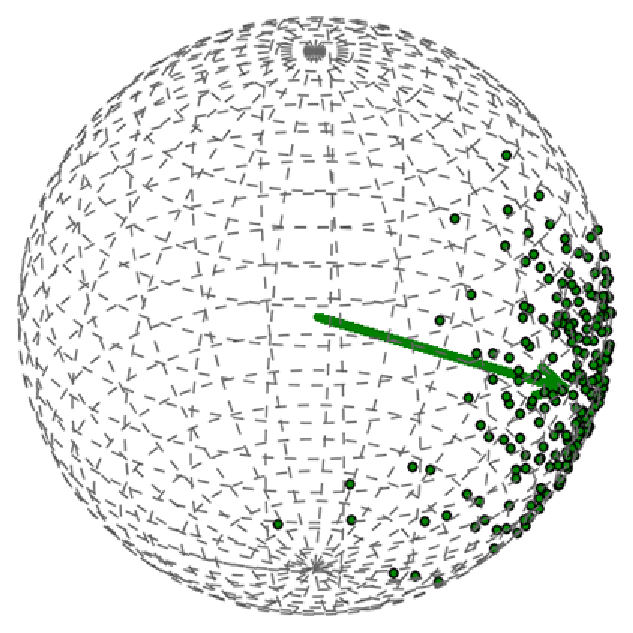
\includegraphics[width=0.8in]{../figures/vf_10.eps}
    \caption{$\kappa=10$}
  \end{subfigure}~
  \begin{subfigure}[b]{0.16\textwidth}
    \centering
    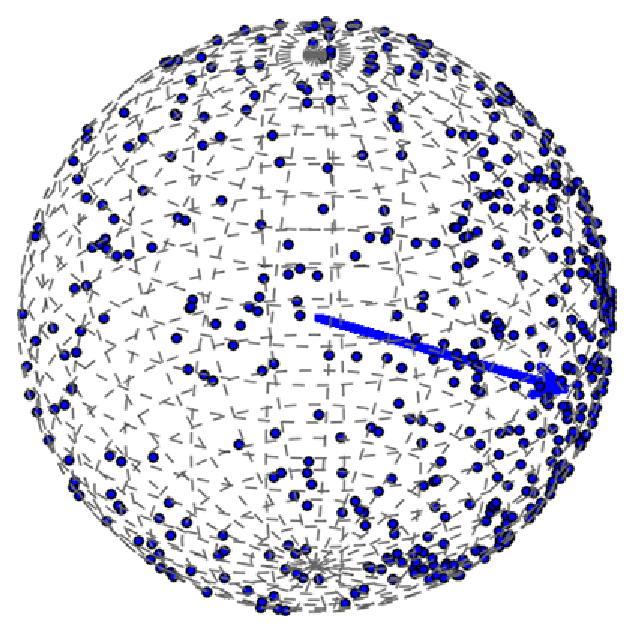
\includegraphics[width=0.8in]{../figures/vf_1.eps}
    \caption{$\kappa=1$}
  \end{subfigure}
  \caption{Points sampled from three von Mises-Fisher distributions on $2$-dimensional spheres with different value of $\kappa$. The mean directions are shown as arrows.}
  \label{fisher}
\end{figure}

In this work, the mean direction $\mu$ of the prior density is given by the previous vector direction ${v_{t - 1}}$. The concentration parameter $\kappa$ is given manually as a constant value.

\noindent\textbf{Observation Density.} We make use of the observation density to characterize local uncertainties, which defines a likelihood function that measures how observations match the current prior model. At step $t$, for a given vector direction $v_t$, the observation density $p({\lambda_t}|{v_t})$ is a conditional density representing how likely the observation $\lambda_t$ measured at position $x_t$ will happen based on the given vector $v_t$. According to the observation $\lambda_t$, the observation density $p({\lambda_t}|{v_t})$ is estimated based on the method presented by Friman et al. in~\cite{frimanTMI06}. We first model the observation matching perfectly to the current state $v_t$ as a distribution $\mu_t$ where the probability of $v_t$ equals to $1$. Then treat $\lambda_t$ as a histogram and let the probability $\lambda_t(i)$ of bin $i$ be an uncertain observation of $\mu_t(i)$, i.e. $\log{\mu_t(i)}=\log{\lambda_t(i)}+\epsilon$. The noise $\epsilon$ can be modeled as additive Gaussian distribution~\cite{Basser1994,Salvador05}, such as $\epsilon \sim N(0,{\sigma ^2}/{\mu _t}{(i)^2})$. Then the observation density, or the likelihood, can be written as
\begin{equation}
  p({\lambda_t}|{v_t}) = \prod\limits_{i = 0}^N {\frac{{{\mu _t}(i)}}{{\sqrt {2\pi {\sigma ^2}} }}} {e^{ - \frac{{{\mu _t}{{(i)}^2}}}{{{2\sigma ^2}}}{{(\log{{\lambda _t}(i)} - \log{{\mu _t}(i)})}^2}}}
\end{equation}

\noindent\textbf{Importance Density.} A usual approach is to use the same distribution as the prior density as the importance function, which is called bootstrap filter or condensation algorithm. However, such importance function may not be always effective, since no observation information is used. As a result, the resulting particles are often outliers of the posterior distribution. Therefore, the observation density is used to determine the $v_t$. Since it is expensive to evaluate the observation density function and there is no need to use the actual observation density as the importance density for the particle filtering method, we choose the observed distribution $\lambda_t$ as the importance density function.
